\documentclass[a4paper,12pt]{report}

% Pakete einbinden
\usepackage[utf8]{inputenc}
\usepackage[T1]{fontenc}

\usepackage{graphicx} % für Bilder
\usepackage[backend=biber]{biblatex} % für Zitate und Literaturverzeichnis
\addbibresource{bibliography.bib}

\usepackage{minted}
\usepackage{fancyvrb}
\makeatletter
\def\minted@verb@delim@a{\do\$}
\makeatother
\usepackage[minted]{tcolorbox}


% Custom JavaScript code box with black border
\newtcblisting{code}{
	listing engine=minted,
	listing only,
	minted language=javascript,
	minted style=colorful,
	minted options={
		linenos,
		fontsize=\small,
		breaklines,
		tabsize=2,
		bgcolor=lightgray!25,
	},
	boxrule=0pt,
	top=0pt, bottom=0pt, left=2pt, right=2pt,
	colback=lightgray!25,
}


% Custom css code box with black border
\newtcblisting{csscode}{
	listing engine=minted,
	listing only,
	minted language=css,
	minted style=colorful,
	minted options={
		linenos,
		fontsize=\small,
		breaklines,
		tabsize=2,
		bgcolor=lightgray!25,
	},
	boxrule=0pt,
	top=0pt, bottom=0pt, left=2pt, right=2pt,
	colback=lightgray!25,
}

% Custom JavaScript code box with black border
% Custom JavaScript code box with black border
\newtcblisting{terminal}{
	listing engine=minted,
	listing only,
	minted language=bash,
	minted style=colorful,
	minted options={
		linenos,
		fontsize=\small,
		breaklines,
		tabsize=2,
		bgcolor=lightgray!25,
	},
	boxrule=0pt,
	top=0pt, bottom=0pt, left=2pt, right=2pt,
	colback=lightgray!25,
}

% Dokumentenbeginn
\begin{document}

% Titelblatt
\title{Open Source Voting Web Application}
\author{Tobias Prasser, Max Martin Hierzer, Gernot Fasching}
\date{\today}
\maketitle

% Abstract
\chapter*{Abstract}
\addcontentsline{toc}{chapter}{Abstract}
\newpage

% Abstract
\chapter*{Kurzfassung}
\addcontentsline{toc}{chapter}{Kurzfassung}
\newpage

% Inhaltsverzeichnis
\tableofcontents
\newpage

% Einleitung
\chapter{Introduction}
Link Gliederung: https://www.diplomarbeiten-bbs.at/durchfuehrung/gliederung-der-diplomarbeit-und-formale-vorgaben
\section{Short description}

The topic of this diploma thesis is creating a platform which supports different voting options like single, multiple or weighted choice. Additionally there should be a Login system with different roles to administer and create or delete polls and one where the user can simply vote for the polls he's included in. Furthermore there an option to disclose the results and who voted for which answers. The database should run on a remote server and be accessed by an API. \\
The reason we chose this topic is because our supervisor is part of the LMP party and they couldn't find an appropriate platform to vote on party intern problems and topics. Hence he approached us and suggested we write our diploma thesis on a voting platform.

\section{Description of performed work}
The aim of this thesis project was to develop an open-source web application that enables organizations to create and mange secure online polls for their members. The platform is designed to be flexible and reusable, so that any group or association interested in running online votes, can benefit from the developed system.\\\\
The Authors of the thesis partnered with Liste Madelein Petrovic(LMP), a political party in Austria, who expressed the need for a platform that offers features not currently available in existing solutions. Their input was especially valuable, as it allowed the team to tailor the application to the real-world needs of a user organization.\\\\
The application includes core features such as poll creation, vote casting, result calculation and a group system. While under active development, the source code is published in a public GitHub repository under the \textbf{MIT License}, ensuring transparency and long-term reusability.\parencite{opensourceinit}
Created an open source voting web application.\\\\
Our aim is to provide a website where different organizations can create and publish polls for their members. Since our finished work will be open source, everyone who wants to create polls will benefit from our work. \\ 

\section{Methodology of the thesis}
This chapter outlines the methodological approach taken during the planning and development of the open-source voting web application. The work was structured around agile software development principles, with a Scrum-inspired workflow that emphasized flexibility, continues feedback and iterative improvement. The development period spanned from early November 2024 to mid-April 2025 with small improvements afterwards, following a planning phase that began in September 2024.\\\\
\subsection{Planning and organization}
The organizational backbone of the project was a GitHub Project board, which was used to manage tasks in the form of issues. Each development sprint was aligned with concrete short-term goals, allowing the team to maintain focused and manageable workload. Some issues were assigned to individual team members, while others, especially more complex features, were shared among multiple developers. The initial planning phase also included the design of the database schema and the selection of a suitable technology stack.\\\\
After careful evaluation, the team chose a backend architecture based on Node.js, Express and Sequelize in combination with a PostgreSQL database. The frontend was built with React and enhanced with Progressive Web App (PWA) capabilities. Before feature development began, the team implemented a basic end-to-end data flow, from frontend input to backend processing, to establish a shared understanding of the system's architecture. Features were then modularized into distinct components to enable parallel development. For example, the single-choice voting feature was split into poll creation, poll display, vote casting, and result visualization.
\subsection{Internal and External Communication}
To support ongoing coordination, the development team held weekly internal meetings via Discord. These meetings served to review current progress, identify technical or organizational blockers and plan subsequent tasks. Each session was documented in the form of written meeting protocols ensure traceability and clarity.\\\\
In addition, the team met with representatives of Liste Madelein Petrovic (LMP) approximately every two to three weeks via Google Meet. These meetings focused on presenting development progress, discussing evolving requirements and jointly prioritizing upcoming tasks. Although the GitHub repository was publicly accessible, the management of the GitHub Project board remained in the hands of the development team. However, during meetings with LMP, open issues were reviewed together and priorities were adapted based on their feedback.
\subsection{Feedback and testing}
One member of LMP regularly tested the application independently and provided direct feedback to the development team. Communication about setup or encountered issues was conducted via a Signal group. This informal yet effective feedback loop allowed the team to adjust functionality in response to real-world usage scenarios. Feedback was especially valuable in evaluating usability and identifying edge cases that might not have been apparent during internal testing.
\subsection{Benefits and challenges}
The adopted methodology brought several advantages. The regular meeting schedule allowed the team to detect and resolve issues early and adapt flexibly to changing requirements. The transparent task management via GitHub facilitated efficient collaboration, even when working remotely or asynchronously.\\\\
However, the collaborative nature of the project also introduced challenges. In some cases, coordination between the development team and the client led to misunderstandings regarding specific requirements or expectations. These were generally resolved through clarification in subsequent meetings, but they underscored the importance of clear and continuous communication in stakeholder-driven projects. 

% Hauptteil
\chapter{Tech Stack}
\section{PostgreSQL}
\subsection{General}
PostgreSQL was selected as the relational database management system for this project due to its balance of performance, reliability, and advanced feature support. Unlike alternatives such as MySQL, MariaDB or SQLite, PostgreSQL offers robust support for complex data types, full ACID compliance and extensibility through custom functions and indexing methods\parencite{postgresdocs}\\\\
While MySQL is widely used, its default configuration prioritizes speed over strict transactional consistency, which may be a drawback for applications requiring high data integrity. SQLite was excluded from consideration because it is more suitable for lightweight or embedded applications and does not support concurrent access by multiple users efficiently.\parencite{postgresvsMysql}\\\\
The installation was also simple because of the detailed install guide provided by multiple sites like \textbf{w3schools}. To create the first database the SQL shell of PostgreSQL was used in the beginning. But due to its excellent tooling support, the open-source tool \textbf{pgAdmin 4} was later used, because it  provided a powerful and user-friendly interface for managing and visualizing the database. Furthermore, the availability of extensive official documentation and community support made it easier to troubleshoot and adapt the database to the project’s needs.\parencite{pgAdmin} \parencite{pgsinstallation}\\\\
\subsection{Database Schema}
The initial design of the database schema evolved significantly during the project as client requirements changed. However, the “Polls” and “Users” tables were identified early on as the foundational entities in the system, with many other tables referencing or depending on them.\\\\
To design and visualize the schema, tools such as \textbf{draw.io} and \textbf{dbdiagram.io} were used, enabling direct import of SQL scripts for entity-relationship diagrams. The final database structure consists of 13 tables. Among these, ”UserPolls”, “UserAnswers”, “PollGroups”, and “QuestionAnswers” serve as intermediary tables that implement many-to-many relationships between core entities.
\begin{figure}[H]	
	\centering	
	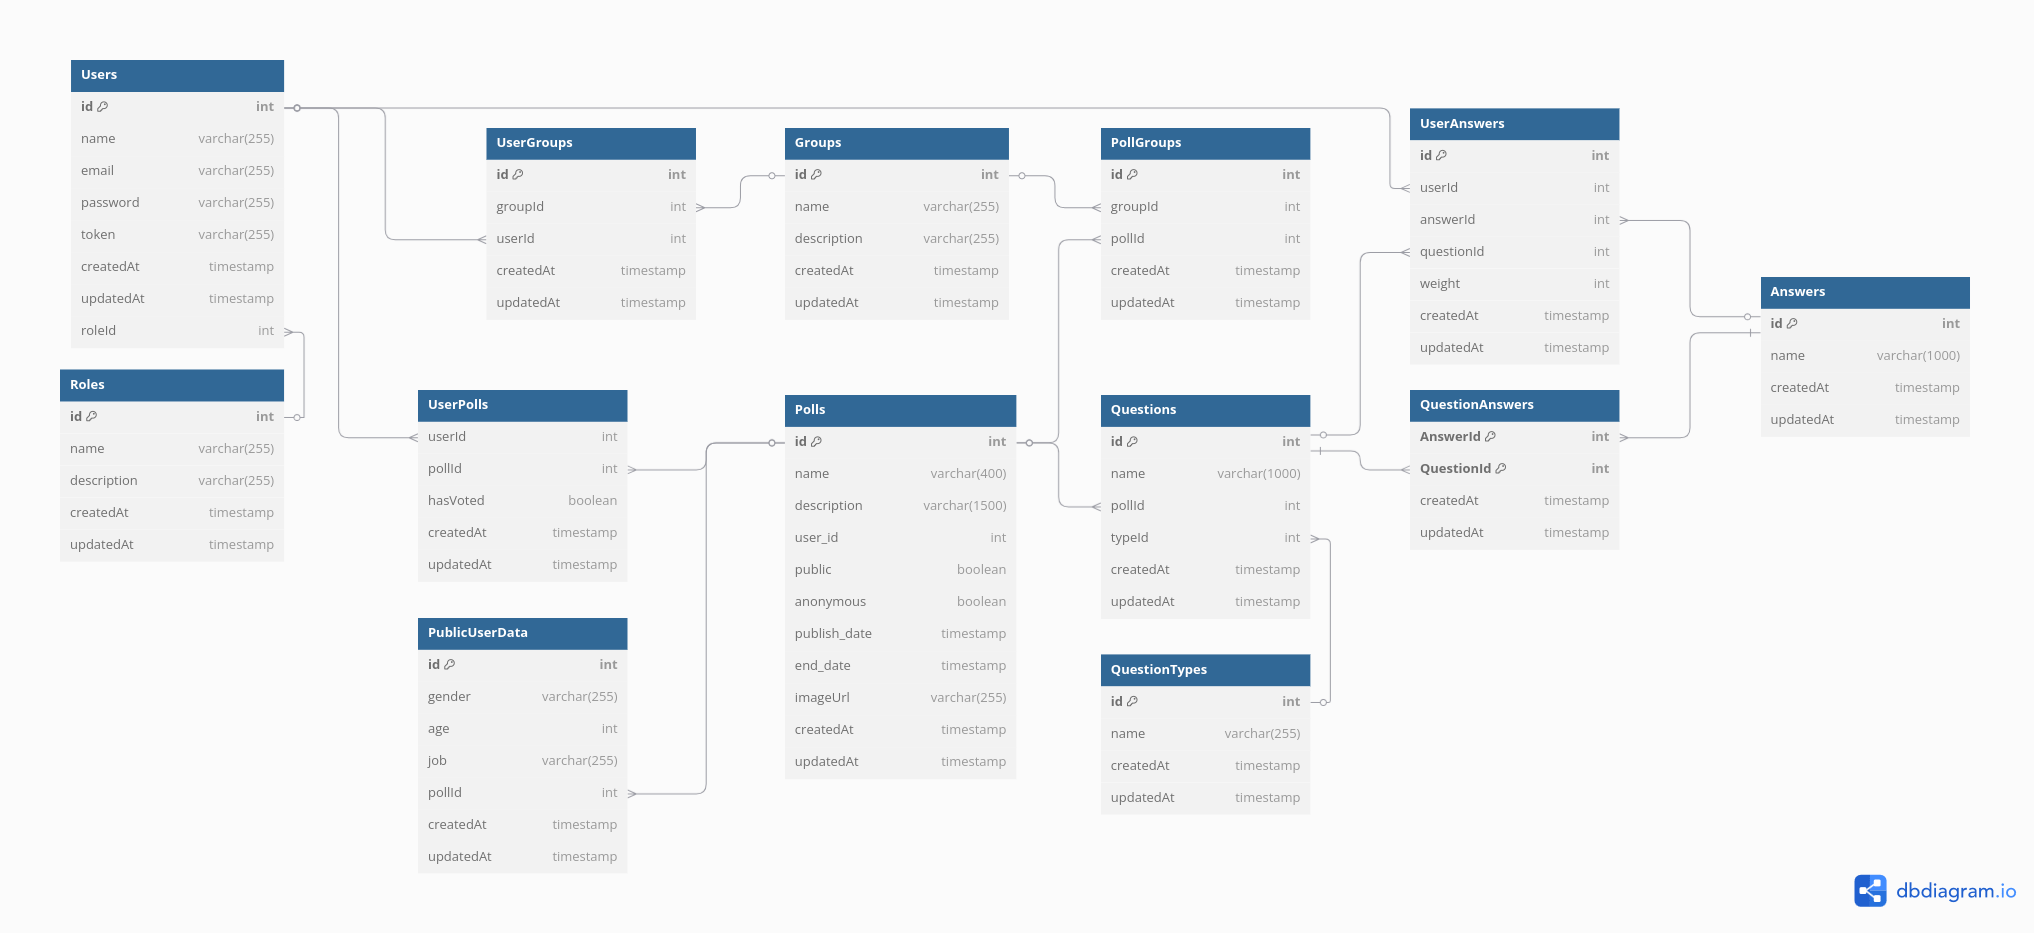
\includegraphics[width=0.8\textwidth]{pics/new_ERD.png}	
	\caption{New Entity Relationship Diagram}	
	\label{fig:new_ERD}
\end{figure}

\section{Node.js}
For the backend \textbf{Node.js} was used. It is a \textbf{JavaScript} runtime environment, that allows the programming language to run on a server instead of the browser. \textbf{Node.js} is based on the V8 engine developed by Google, which compiles \textbf{JavaScript} into machine code for faster execution.\parencite{nodejs-intro}\\\\
\subsection{Advantages}  
One of the main advantages of \textbf{Node.js} is its non-blocking I/O model. This means it does not wait for certain processes, such as reading from a file or a database, to finish before continuing with other operations. Instead, it starts a process and immediately listens for the next event. When the initial process finishes, a callback function is executed. This makes it possible for \textbf{Node.js} to handle multiple operations concurrently, even though it is inherently single threaded. This results in high performance and responsiveness.\parencite{nodejs-nonblocking}\\\\
Another advantage of \textbf{Node.js} is that it creates a \textbf{unified language environment} because both the frontend and the backend can be programmed in \textbf{JavaScript}. This simplifies the development process, improves code reusability, and reduces the learning curve, since developers do not need to learn an entirely different programming language for the backend.\\\\
\textbf{Node.js} also has the \textbf{Node Package Manager} (\textbf{npm}) which provides access to a vast collection of reusable packages and modules. These include pre-built code solutions to simplify common requirements like encryption and also sending emails, both of which where used in this project.\parencite{mdn-express-nodejs}


\section{Sequelize}
Sequelize was selected as the Object-Relational-Mapping(ORM) tool for this project due to its seamless integration with Node.js and PostgreSQL, offering a robust and declarative approach to database interaction. By abstracting raw SQL queries into model-based definitions, Sequelize enables a more maintainable and readable codebase, especially in a project with complex data relationships and evolving schema requirements.\\\\
Its support for model associations, transaction management and migrations provides a powerful foundation for implementing scalable and consistent backend logic. Additionally, Sequelize's promised-based architecture aligns well with asynchronous programming paradigms common in modern JavaScript applications, improving performance and responsiveness.\parencite{sequelizegit}\\\\
The comprehensive documentation, active community support, and compatibility with various SQL dialects, as in our case PostgreSQL, further contributed to the decision to use Sequelize as the ORM in this project.\\\\
When compared to other ORMs like Prisma, Sequelize offers a mature and stable solution with wide database compatibility and a strong community. While Prisma provides a modern, type-safe approach with auto-generated types, Sequelize's straightforward API and extensive features make it a reliable choice for this project, because of its simplicity and flexibility.\parencite{Ormcomparemedium}\parencite{Ormcomparedhiwise}

\section{Express.js}
Express.js is a flexible web framework for Node.js which is widely used for building RESTful APIs. It provides a middleware-based architecture that allows for clear routing, request handling, and modular code organization. In this application. Express serves as the backend framework that handles HTTP requests to handle communication between the frontend and the database. \cite{expr-base} \\ \\
There are multiple alternative frameworks that were evaluated in the selection process:
\paragraph{NestJS} provides a structured and scalable framework based on TypeScript. The ideal use for NestJS would be a large enterprise project, which this thesis is not. This adds complexity and a way steeper learning curve, which is why this option was not chosen. \cite{expr-comp}\cite{expr-comp2}\cite{nest-js}
\paragraph{Fastify} is a performance-orientated alternative to Express.js, which even outperforms it. However, since this framework is less mature, there is less documentation and a smaller community for support in comparison to what Express.js is offering. Since the developers of this thesis had no real experience with APIs the more developer-friendly Express was chosen over Fastify. \cite{expr-comp} \cite{expr-comp2} \\ \\
Another option is Hono, which is a new ultra-lightweight framework, but is still niche and lacks in support and documentation, which is why Express was favored. FeatherJS is built on Express, designed for real-time applications. Since real-time features were not needed for this platform, FeatherJS was not chosen. \cite{expr-comp} \cite{expr-comp2}
\subsection{Architecture}
The backend is organized into the following layers:
\begin{itemize}
	\item \textbf{Routing Layer:} This layer defines the application's HTTP endpoints and maps incoming requests to the appropriate controller functions. Routes are grouped thematically using \verb|express.Router| (e.g., \verb|/api/users|) to maintain modularity and logical organization.
	
	\item \textbf{Controller Layer:} Controllers serve as intermediaries between the routing layer and the business logic. They are responsible for extracting relevant data from incoming requests, invoking the necessary service functions, and constructing structured responses. This ensures that request handling remains concise and focused.
	
	\item \textbf{Service Layer:} This layer contains the main application logic and performs database operations using \texttt{Sequelize}. Each service function handles one use case, such as creating a user or poll. Data access is performed directly within the service layer.
\end{itemize}
\subsection{Error Handling}
In the Express.js backend, the error handling for the application is integrated directly into the controllers. The controller interacts with the service layer and handles HTTP requests. 
\begin{figure}[H]
	\begin{code}
		const editController = {
			async updatePoll(req, res) {
				try {
					const updatedPoll = await editService.updatePoll(req.body);
					res.json(updatedPoll);
				} catch (error) {
					res.status(500).json({ error: error.message });
				}
			},
		};
	\end{code}
	\caption{Example of error handling in controller}
	\label{fig:controller-err}
\end{figure}
In the code above, the updatePoll function attempts to handle errors using a try/catch. When an error occurs during the execution of the updatePoll service function, the error is caught in the catch block. The server then responds with a 500 Internal Server Error status, including the error message in the response body. This ensures that the client is informed about the failure. This is the most basic form of error handling and can be improved in the future e.g. by using specific errors like "400 Bad Request" or "404 Not Found" instead of the simple "500 Internal Server Error" to give a more detailed description to the client. 
\subsection{CORS}
In the application, Cross-Origin Resource Sharing (CORS) is managed using the cors middleware in Express.js. CORS is a security feature implemented by web browsers that controls how web pages from one domain can make requests to a backend server hosted on another domain. It is particularly important when the frontend and backend are hosted on different origins, such as when they are running on different ports during development or on different subdomains in production. \\ \\
In this case, CORS is configured with the default settings, meaning that the backend allows cross-origin requests from any domain. This default setup permits all HTTP methods (like GET, POST, PUT, DELETE, etc.) and headers from any origin, making it very permissive. This configuration is helpful during the development phase, as it avoids the need for specifying which domains or methods are allowed. \\ \\
However, while the default configuration is useful in development, it is not recommended for production environments due to security concerns. Allowing any origin to interact with the backend can expose the server to potentially malicious requests from untrusted sources. It is generally better to restrict CORS to specific trusted domains and limit the allowed HTTP methods and headers to only those necessary for the application. Therefore, this should be improved in the future. \cite{mdn-cors}

\section{React.js}
React.js is a declarative. component-based JavaScript library, which is widely adopted in modern web development due to its modular structure and virtual DOM optimization. In this application, React is used as the frontend framework responsible for rendering the user interface, managing local and global state, and communicating with the backend API. \cite{react-docs}\\
Several alternative frameworks were taken into consideration during the selection process:
\paragraph{Vue.js} offers a simple and intuitive syntax that would lower the learning curve for new developers. However, since React has a larger ecosystem, widespread community support and a better compatibility with third-party libraries, it was chosen over Vue. \cite{react-docs} \cite{vue-docs} \\ \\
\paragraph{Angular} is a comprehensive frontend framework with built-in support for routing and forms. While powerful, Angular is way more complex and is harder to learn which is why React was preferred for the scope of this project. \cite{angular-docs} \\
Besides these two, smaller frameworks like Svelte were also considered, but due to smaller communities and less comprehensive documentation they were not chosen. Another reason why React was the preferred framework is because the developers were already familiar with the Syntax and used it for small exercises on various platforms like "freecodecamp.org".
\subsection{Architecture}
React.js is based on a component oriented architecture, where the user interface is broken down into small, reusable building blocks called components. Each of these is typically a function that returns a declarative description of how the UI should look like, using JavaScript XML (JSX). Every component also manages its own internal logic and state, responds to user interaction and renders the content dynamically. \\
React components receive configuration and data through props, which are passed from the parent component. They can also manage they internal state using React's "Hooks API", such as "useState" and "useEffect" for handling effects like data fetching. \cite{react-docs} \cite{mdn-react}

\section{PWA}
The application is \textbf{PWA}, \textbf{Progressive Web App}, compatible.
\subsection{Function}
“A progressive web app (PWA) is an app that's built using web platform technologies, but that provides a user experience like that of a platform-specific app.”
This makes it possible to combine the best features of both websites and platform-specific apps.\parencite{mdn-pwa}\\\\
\subsection{Function Platform-Specific}
These types of applications are developed only for a particular operating system, which means that the code written can not be, at least not all of it, reused for other systems. The biggest target platforms for those applications are \textbf{Android} and \textbf{IOS}.\\\\
Because they are tailored to the system they provide several advantages:

Therefore \textbf{PWAs} can run on multiple platforms just like websites, but also retain the ability to run offline and in the background like platform-specific apps.

\chapter{Features}

\section{Login}
The login feature is essential for our application, as users need a secure and reliable way to authenticate themselves and gain access to their accounts. It consists of two main functionalities: the login itself and also the logout. Additionally, we have implemented user-friendly error handling to enhance user experience as well as security.
\subsection{Frontend}
The frontend component of the login feature uses React's built-in useState hook in order to manage the input username and password and store them in the component's state temporarily. After submitting the login form, the input data is sent to the backend API via a POST request.\\\\
The password is sent to the backend in plaintext over HTTPS. It is not encrypted on the client side, because HTTPS already provides built-in encryption and also protects against interception or man-in-the-middle attacks.
\subsection{Backend}
The backend receives the login request through a predefined API route that forwards the data to the handleFetchLogin function in the user controller. It extracts the username and password from the request body and passes them to the fetchLogin function in the user service.\\\\
This function first checks if a user with the provided username even exists in the database. If no user is found, it returns an error message stating that either the username or password is invalid. We intentionally chose to not specify which of the two parts is incorrect in order to prevent attackers from being able to determine whether a username exists in the system. This provides protection against user enumeration attacks.\\\\
If a user is found, the provided password is then compared to the hashed password stored in the database using bcrypt's comparison method, bcrypt.compare(). In case the passwords do not match, the same error message mentioned above is returned to the frontend.\\\\
However, if the password is correct, the backend returns a response containing a success indicator, the user's unique ID (userId), their username, the assigned role ID (roleId), and the name of the role (roleName).
\subsection{Error Handling and Security}
Error handling is implemented consistently across both frontend and backend to ensure security and user-friendliness. If a login attempt fails, whether due to an incorrect username, password, or both, the system always returns the same general error message. This prevents attackers from determining whether a specific username exists in the system.\\\\
Sensitive data like passwords is handled securely. Passwords are not stored in plain text. Instead they are hashed using bcrypt before being inserted into the database. Furthermore, communication between frontend and backend is encrypted through HTTPS. This ensures that all transmitted data remains private and protected from unauthorized access.

\section{Registration}
The application features a controlled and secure registration. In order for users to be able to join the system, they first have to be invited. The registration consists of two main functionalities.
\subsection{Admin Registration Process}
Only administrators are allowed to invite new users. They start the process by navigating to the registration tab and entering the user's email as well as their intended role. After submitting, the data gets sent to the "sendEmail" function in the backend through a POST request.\\\\
The function checks if a user with the provided email address already exists in the database. If so, it returns a message indicating exactly that. In case the email is not found, an invitation email is sent and a new user entry with the provided email, role ID and a randomly generated token is created. The token is later used for verifying the legitimacy of the registration. If the process is successful the administrator is informed that the email was sent and the user was created successfully.
\subsection{User Registration Process}
The email sent to the user contains a registration link consisting of the URL of the application and the previously mentioned token. By clicking the link, the user is redirected to a registration page on which they can enter a username and password.\\\\
The page contains three fields. One for the username, one for the password and one for password validation. This approach was chosen in order to ensure a correct password input. If the contents of the two password fields do not match, an error message telling them about the mismatch is displayed. Similarly, if any of the fields are left blank, submission is disabled and the user is notified of the problem. If all inputs are valid the token extracted from the link, as well as username and password are sent to the backend using a PUT request. The password is sent in plain text over HTTPS, as explained in the login section above.\\\\
The backend then passes the data to the "createUser" function. It first checks whether the token exists in the database and also if the username is already being used. In both cases, no token or existing username, the user receives an error message telling them the specific problem. If the username is the issue they can just change it and try again, but if it is the token it will never work no matter how often they retry. If both checks pass, the password is hashed using bcrypt's hash function. The database is then updated with the new username and hashed password. The token is set to null to prevent reuse. If everything is successful the function returns a success message is returned telling the user that the registration is complete. After five seconds they are redirected to the login page, where they can then log in and use the application.
\subsection{Sending Invitation Emails}
For automatic sending of the invitation emails, we implemented two different approaches. Therefore both will be explained below.
\subsubsection{Nodemailer (SMTP)}
The first approach uses "nodemailer" to send emails over SMTP. Firstly a transporter is created using nodemailer's "createTransport" function. There several options can be defined including the host, like gmail or a custom SMTP server, the port, secure option and also authentication credentials. 
\begin{figure}[H]
	\begin{code}
		let transporter = nodemailer.createTransport({
			host: "smtp.mailersend.net",
			port: 587,
			secure: false,
			auth: {
				user: test.email@domain.at,
				pass: Password1,
			}
		});
	\end{code}
	\caption{This is an example for the transporter using mailersend as the SMTP server}
	\label{fig:beispielcode}
\end{figure}
After setting up the transporter, the email options are defined. These include the sender and recipient addresses along with the subject and general content of the email.
\begin{figure}[H]
	\begin{code}
		const mailOptions = {
			from: "Tool" <test.email@domain.at>,
			to: user@email.at,
			subject: "Polling tool",
			text: "Hello this is your invitation."
		};
	\end{code}
	\caption{This is an example for the email options}
	\label{fig:beispielcode1}
\end{figure}
Finally the email is sent using "transporter.sendMail(mailOptions)".
\subsubsection{MailerSend API}
The second approach uses the MailerSend API to send the invitation emails. This method was implemented because our deployment host blocks all SMTP ports.\\\\
To use the MailerSend API, a transporter is created with "new MailerSend" and the API key. Just like int the first method mail options are created specifying the sender, recipient, subject and message.
\begin{figure}[H]
	\begin{code}
		const mailOptions = new EmailParams()
		.setFrom(new Sender(test.email@domain.at, "Tool"))
		.setTo([new Recipient(user@email.at)])
		.setSubject("Polling tool")
		.setText("Hello this is your invitation.");
	\end{code}
	\caption{This is an example for the email options for MailerSend}
	\label{fig:beispielcode2}
\end{figure}
The email is then sent using "mailerSend.email.send(mailOptions)".
\subsection{Roles}
Implementing a role-based system with three distinct roles - "Admin", 
"Poweruser", and "Normal" - is crucial for the functionality and security of the application. By assigning permissions flexibly, a clear hierarchy is established, enhancing both user experience and data integrity. Admins are granted full control over the application, while Poweruser enjoy extended privileges for managing polls. Normal users can seamlessly participate in polls and view results without jeopardizing sensitive functionalities. This structure facilitates efficient task delegation and scalability, allowing the application to be easily expanded with additional roles  in the future. The role system thus significantly contributes to the security, organization, and user-friendliness of the polling application.\\\\


This functionality was implemented by introducing a "Roles" table, which maintains a one-to-many relationship with the "Users" table. Each user is associated with a specific role through the foreign key \textbf{roleId}. The roles are defined and manged exclusively within the database, with the following ID assignments: 1 for administrators, 2 for powerusers and 3 for standard users. Role-based access is determined solely based on these database-level associations.\\

\section{Group System}

The group system was implemented to simplify user management. By grouping users together, poll creators can efficiently control access to polls. Instead of managing individual users, a poll owner can assign entire groups to a poll, ensuring that only selected users can participate in voting. \\ \\
Beyond restricting access, the system also allows assigning different permission levels. Users with elevated privileges—such as power users or administrators—can be granted editing rights, enabling collaborative management of polls. Additionally, poll results are only visible to users belonging to groups that have access to the poll. \\ \\
To support the group system, a new navigation option was added to the interface. The page for creating groups is shown in Figure~\ref{fig:create_groups}. At the top of the page, a toggle button labeled \textit{Gruppen Bearbeiten} allows switching between group creation and editing. Below that, users can enter a group name and provide a short description explaining the group's purpose and membership.
\begin{figure}[H]
	\centering
	\includegraphics[width=0.8\textwidth]{pics/create_groups.png}
	\caption{Create Groups Page}
	\label{fig:create_groups}
\end{figure}
At the bottom of the form, a React Select component is used to assign users to the group. The group editing interface is visually similar to the creation interface, with the addition of a group selection dropdown and a removal option for existing members. An additional feature of the editing interface is the ability to export group members, allowing external tools to be used for planning and organization.

\subsection{Backend}

To support the group functionality on the backend, three new database tables were introduced:

\begin{itemize}
	\item \textbf{UserGroups}: Represents a many-to-many relationship between \textbf{Users} and \textbf{Groups}. It stores user assignments to groups and is essential for frontend group management.
	\item \textbf{Groups}: This table is the core of the group system, storing group metadata such as name and description.
	\item \textbf{PollGroups}: Establishes a many-to-many relationship between \textbf{Groups} and \textbf{Polls}. It defines which groups have access to which polls and is directly used in the poll creation and editing workflows. \\
\end{itemize}
When displaying polls to a user, the system queries all groups the currently signed-in user belongs to and checks whether any of those groups are assigned to a poll. This determines the user's access to view or interact with a poll.

\subsection{Frontend}
The frontend for the group system on the group page includes several key elements already mentioned:
\begin{itemize}
	\item \textbf{Toggle Mode:} A button labeled \textit{Gruppen Bearbeiten} allows switching between group creation and editing modes without navigating away from the page.
	\item \textbf{Form Inputs:} The interface includes input fields for entering the group name and description. These are controlled components in React, ensuring real-time validation and state management.
	\item \textbf{User Selection:} The user assignment is implemented using a React Select component, which allows searching and selecting users from a dropdown. In editing mode, an additional select dropdown is displayed to remove existing users from the group.
	\item \textbf{User Export:} In editing mode, an export function is available, allowing the list of group members to be downloaded. This can be useful for external planning or documentation.
\end{itemize}
In addition to group management, a React Select component is also integrated into the poll creation and editing sections. Here, users with editing privileges can assign groups to a poll or remove them. This ensures that only selected groups have access to vote or view the poll. \\ \\
Overall, these features provide a smooth and efficient user experience while significantly reducing the administrative effort required to manage poll access.

\section{Create Polls}
The \textbf{Create Polls} section represents the poll creation interface of the system. It allows users to create customized polls based on their needs. Customization options include entering a poll name and description, selecting different poll types, assigning the poll to specific groups, defining a start and end date for the voting period, uploading an image and dynamically adding questions with chosen question types and a variable number of answers per question.
\subsection{Error Handling}
To ensure that polls are created correctly and without missing information, the \textbf{Create Polls} section includes validation in the frontend and transaction in the backend.
\subsubsection{Frontend}
In the frontend, validation is handled by the \textbf{validatePollData} function located in a separate file, \textbf{ValidatePolls.js}. This function checks wether any required input fields are left empty. If a required field is empty, a specific message about which field is afflicted is returned, which is then displayed to the user. This improves the user experience and also prevents unnecessary API calls to the backend.
\begin{figure}[H]
	\begin{code}
		validatePollData(poll, publishDate, endDate, questions) {
			if (!poll) return `Poll name is required`;
			if (!publishDate) return `Publish date is required`;
			if (!endDate) return `End date is required`;
			
			for (let questionIndex = 0; questionIndex < questions.length; questionIndex++) {
				if (!questions[questionIndex].name) return `Question ${questionIndex + 1} requires text`;
				for (let answerIndex = 0; answerIndex < questions[questionIndex].answers.length; answerIndex++) {
					if (!questions[questionIndex].answers[answerIndex].name) return `Answer ${answerIndex + 1} in Question ${questionIndex + 1} requires text`;
				}
			}
			return null;
		}
	\end{code}
	\caption{Frontend validation function for poll creation}
	\label{fig:beispielcode2}
\end{figure}

\subsubsection{Backend}
Even though validation already occurs in the frontend, the backend still needs to ensure that all database insertions are executed correctly. This is handled in the \textbf{createPoll} function. To maintain data integrity, database transactions are used.\\\\
A transaction is created and used for all data operations involved in poll creation, including inserting the poll, its questions and all corresponding answers. Once all operations are completed successfully, the transaction is committed. If any error occurs during the process, the transaction is rolled back, undoing all previous changes made during that transaction. This ensures that no incomplete data is saved into the database.
\begin{figure}[H]
	\begin{code}
		try {
			const transaction = await sequelize.transaction();
			const createdQuestion = await Question.create({
				name: question.name,
				pollId: createdPoll.id,
				typeId: questionType.id,
			}, { transaction });
			await transaction.commit();
		} catch (error) {
			await transaction.rollback();
		}
	\end{code}
	\caption{This is an example for the transaction usage}
	\label{fig:beispielcode2}
\end{figure} 
\subsection{Start-/ Endtime}
To make Polls more manageable, users can define a voting period by setting a start and end time during poll creation. This feature consists of two main parts.
\subsubsection{Setting The Times}
The first part involves setting the start and end time in the poll creation interface. Initially, the HTML native input type \textbf{datetime-local} was used. However it was not fully supported by every browser, including Firefox which could only depict the date but not the time. For this reason, after some consideration, the "react-datetime" component was chosen instead.\\\\
When a user clicks on the input field, a graphical selector appears, which allows the user to select both the date and time easily.\\\\
Once the poll is submitted, the selected start and end times are sent to the \textbf{createPoll} function in the backend via a POST request. There, the received times are converted to JavaScript \textbf{Date} objects before being inserted into the database.
\subsubsection{Utilizing The Times}
These time-based conditions are the core feature used to differentiate between the various states of a poll: edit, voting, and results. To apply these conditions, three arrays are created—each corresponding to one of the states—and passed as props to their respective React components.  
Figure~\ref{fig:timeuti} shows the code that performs this classification. The \texttt{data} variable contains all polls retrieved from the database via an API call. The \texttt{current\_datetime} is set using \texttt{new Date().toISOString()}. The function iterates through each poll, comparing its \texttt{publish\_date} and \texttt{end\_date} to the current time.

A poll is:
\begin{itemize}
	\item pushed into the \texttt{edit} array if the current time is earlier than its \texttt{publish\_date},
	\item added to the \texttt{vote} array if the current time is between \texttt{publish\_date} and \texttt{end\_date} and the poll is not public,
	\item moved to the \texttt{results} array if it is public and its \texttt{end\_date} has already passed.
\end{itemize}

An important detail is how \textit{public polls} are handled. Since they are not intended to appear in the standard voting view, they are excluded from the vote array. In contrast, public polls may appear in the results view even before their end date, allowing creators and interested parties to observe the vote development in real time.


\begin{figure}[H]
	\begin{code}
		data.forEach((poll) => {
			if (poll.publish_date > current_datetime) edit.push(poll);
			else if (poll.publish_date <= current_datetime 
			&& poll.end_date >= current_datetime 
			&& poll.public === false) vote.push(poll);
			else if (poll.public === true && poll.end_date < current_datetime) results.push(poll);
		})
	\end{code}
	\caption{Sorting the polls depending on time}
	\label{fig:timeuti}
\end{figure}
\subsection{Poll Image}
In response to client requirements, a feature was implemented allowing users to upload a title image for each poll. This image serves a purely atmospheric and aesthetic purpose, aiming to enhance the visual appeal of the poll and provide users with a more engaging and intuitive introduction to the survey topic. By incorporating visual context, the feature helps draw user attention and encourages participation, particularly in cases where the subject matter benefits from visual reinforcement.\\\\
\subsubsection{Backend Implementation}
On the backend, the image upload is handled using the \textbf{multer} middleware in the \textbf{imageRoutes.js} file. The storage engine is configured to save uploaded files in the \textbf{uploads} directory with a unique filename based on a timestamp and the original file extension. The file types are restricted to JPEG, PNG and GIF formats through a custom file filter to ensure consistency and security.\parencite{expressmulter}
\begin{figure}[H]
	\begin{code}
		const storage = multer.diskStorage({
			destination: (req, file, cb) => {
				cb(null, 'uploads');
			},
			filename: (req, file, cb) => {
				cb(null, Date.now() + path.extname(file.originalname));
			}
		});
	\end{code}
	\caption{Custom storage engine configuration for multer}
	\label{fig:multer_config}
\end{figure}
The route \textbf{/api/upload-image} is exposed via the Express router and returns the public URL of the uploaded image on success. The image can later be used as part of the poll metadata.\\
In \textbf{app.js}, static file serving is enabled for the \textbf{uploads} directory to make the images accessible to the frontend:
\begin{figure}[H]
	\begin{code}
		app.use('/uploads', express.static('uploads'));
	\end{code}
	\caption{Static file serving enabled}
	\label{fig:static_file_serving}
\end{figure}
\subsubsection{Frontend Integration}
On the frontend, the image upload is handled within the \textbf{CreatePolls.js} component. When a user selects an image file, the \textbf{handleImageUpload} function is triggered. 
\begin{figure}[H]
	\begin{code}
		const handleImageUpload = async (event) => {
			const file = event.target.files[0];
			if (!file) return; 
			const previewUrl = URL.createObjectURL(file);
			setImage(previewUrl);
			const formData = new FormData();
			formData.append("image", file);
			try {
				const res = await fetch(`${process.env.REACT_APP_API_URL}/api/upload-image`, {
					method: 'POST',
					body: formData,
				});
				const data = await res.json();
				if (res.ok) {
					setImageUrl(data.imageUrl); 
				} else {
					setResponse('Error uploading image');
				}
			} catch (error) {
				console.error('Error uploading image:', error);
				setResponse('Error uploading image');
			}
		};
		
	\end{code}
	\caption{handleImageUpload function}
	\label{fig:handleImageUpload}
\end{figure}
This function performs the following steps.
\begin{enumerate}
	\item A local preview of the selected image is created using the browser's \textbf{URL.createObjectURL()} method. This provides immediate feedback to the user by displaying the image in the form before it is uploaded.
	\item To prepare the image for upload to the server, a new instance of the \textbf{FormData} object is created. This object is specifically designed to handle form submissions that include binary data such as files. The use of \textbf{FormData} is necessary because standard JSON-based payloads \textbf{application/json} do not support file transfers. The browser automatically sets the \textbf{Content-Type} to \textbf{multipart/form-data} when \textbf{FormData} is used, which is the appropriate MIME type for file uploads.
	\item The image is uploaded to the backend by making a \textbf{POST} request to the endpoint \textbf{api/upload-image}. If the upload is successful, the backend responds with the relative path to the stored image, which is then saved in the component state \textbf{imageUrl} for use in the final poll submission.
	\item The uploaded images's URL is included as part of the final poll payload when the user submits the form. This allows the backend to store the image reference in the database alongside the poll data.
	\item Upon successful poll creation, the image preview, image URL and file input are all reset to ensure a clean state for subsequent poll creation actions.
\end{enumerate}
By combining real-time preview functionality with reliable backend integration, the image upload feature significantly improves the overall usability and aesthetic appeal of the application.
\subsection{Questions}
To support a variety of survey use cases, the system offers three types of questions: single choice, multiple choice, and weighted choice. Each type serves different purposes and allows for more flexible poll creation depending on the information being collected. The differences and use cases for each question type are described in the following section.
\subsubsection{Single Choice}
Single choice questions are the simplest type of question in the system. They allow users to select exactly one option from a list of possible answers. One major benefit of this question type is the minimal time required to answer. Deciding on a single option is usually faster than selecting multiple answers or assigning weights. \\ \\
Another advantage is the simplicity of data analysis. Since each user provides only one answer, the resulting data is easier to aggregate and interpret compared to other question types. This format is particularly effective when the poll creator wants to highlight the most important user preferences. A single choice question forces participants to choose the most relevant option, thereby focusing the collected data on the most impactful areas. \\ \\
However, limiting users to one response can also lead to incomplete or skewed data, especially in cases where the question is ambiguous or multiple answers would apply. In such scenarios, forcing a single choice may result in user frustration or less accurate feedback. \cite{singlevsmultiple} \\ \\
Figure \ref{fig:singlechoice} shows an example of a single choice question in the voting section. The options are presented using radio buttons, ensuring that only one answer can be selected at a time.
\begin{figure}[H]	
	\centering	
	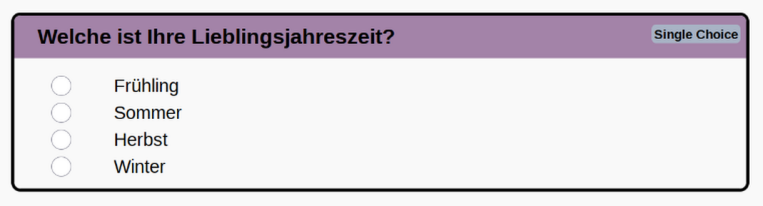
\includegraphics[width=0.8\textwidth]{pics/Single_Choice.png}	
	\caption{Single Choice Vote}	
	\label{fig:singlechoice}
\end{figure}
\subsubsection{Multiple Choice}
Multiple Choice questions, also known as multiple response questions allow users to select one or several answers from a given list of options. This question format offers flexibility in collecting diverse user options, as participants are not restricted to a single choice. It is especially usefull when multiple options may be valid or relevant from a participant's perspective.\\\\
In contrast to single choice questions, multiple choice provides a richer insight into the perspective of the user when more than one answers can be picked. In the application's voting interface, multiple selections are implemented by enabling checkboxes for each answer option. When this question type is rendered, users can check or uncheck any combination of available responses except unchecking all answers.\\\\
\subsubsection{Weighted Choice}
In weighted choice questions, users select one answer from a set of predefined options and assign an importance level to their choice using a scale from one to nine.\\\\
This question type gives more insight into preferences than single or multiple choice questions, because poll participants not only select which answer they prefer, but also indicate how important it is for them. As a result, it becomes easier to decide wether an issue should be prioritized or not.\\\\
The importance scale is implemented as a custom designed component consisting of nine buttons, each representing a value from one (least important) to nine (most important). If the question type is weighted choice, this scale is displayed along with the standard single choice option.\\\\
\subsection{Demographic Questions}
To gather the data of our public voters, the implementation of demographic questions was crucial. This feature is only available for public polls since the created user would be part of the organization using our project and therefore have the data already. If the users is not part of the organization there is still the option to contact them via the e-mail used for the registration. Since most of these questions are similar for every poll, a modular system where questions can be created, added, removed and changed is the best solution. Figure \ref{fig:create_dem_que} shows the demographic question in create polls. The options and functionality of these questions are the like ones described in the previous sections, with the difference that weighted is not an option, since demographic data is more like a fact less an opinion.
\begin{figure}[h!]
	\centering
	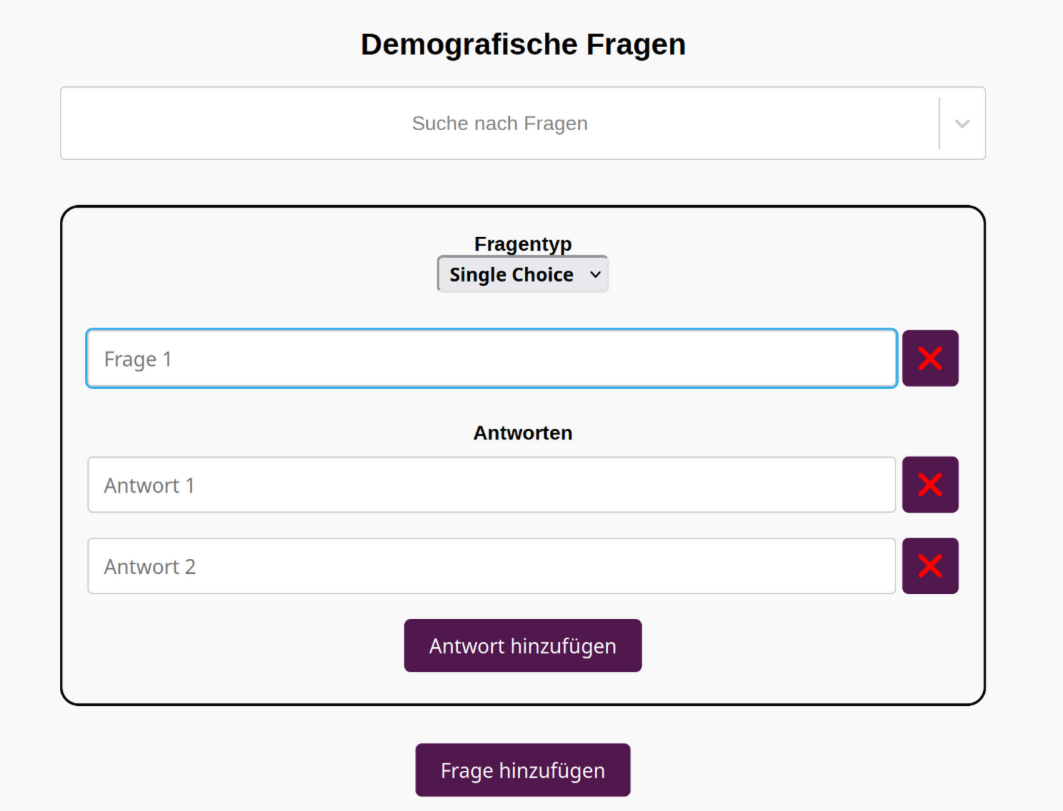
\includegraphics[width=0.65\textwidth]{pics/demographic_question_create.jpg}
	\caption{Create Demographic Question}
	\label{fig:create_dem_que}
\end{figure}
\\
The new part for this feature is the search bar. For this the "Select" component of "react-select" is used. The components' controllable state props and modular architecture allows  "isMulti" to select multiple options or "isSearchable" to search. These features, allow easy implementation and an already styled search bar in the project. \parencite{reactselect}
\\ \\
The database structure for the demographic questions is similar to the standard ones. The table "PublicQuestions" is used to store the question specific data like name and type. To enable the reuse of questions on different polls "PublicQuestions" is in an many-to-many relationship with "Polls" through "PublicPollQuestions". Answers are stored within the table "PublicAnswers", which is connected to "PublicQuestions" via "PublicQuestionAnswers. This relation is also many-to-many since the options yes or no for example would be used in multiple questions. 
\\ \\
For the select every existing question with its answers is fetched from the database and stored within an array. The options are then mapped with the value being id and the label as name of each element. To display the selected options they are mapped through and use the same functions as the standard ones used for the poll. When saving these questions a problem arises, as the selected ones are already stored in the database and possibly changed. To handle this a findOrCreate \ref{fig:publicQuestions} is used to get the existing questions and answers or create new ones. This function also returns each instance found or the created one. With this the question and answer ids can be used for the many-to-many relationship. \parencite{sequelizedoku} 
\begin{figure}[h!]
\begin{code}
let [createdQuestion, created] = await PublicQuestions.findOrCreate({
	where: {
		name: question.name,
		typeId: questionType.id,
	}
});
\end{code}
	\caption{findOrCreate PublicQuestions}
	\label{fig:publicQuestions}
\end{figure}

\section{Edit Polls}
Editing a poll is essential for maintaining a smooth administrative workflow on the platform. Editing is only permitted before the poll is published — the concept of publish time is already described in the creation section. Without this feature, power users and administrators responsible for creating polls would encounter significant limitations. \\ \\
For instance, simple issues such as typos or unclear instructions could not be corrected, requiring the entire poll to be deleted and recreated. Additionally, the edit functionality enables collaborative poll creation: one user can create the initial poll and assign a group with editing privileges. These users can then revise the poll, allowing for a structured and collaborative workflow. Furthermore, setting the publish time to a future date ensures that the team has ample time to discuss and refine the poll before it goes live.
\subsection{Backend}
The backend for editing uses the same structural approach described in the creation section. However, specific logic is implemented to handle operations such as adding, updating, and removing elements of an already created poll. The complete poll data is sent from the frontend via the API, and the backend separates and processes it accordingly. \\ \\
Before applying any changes, the backend checks whether the poll has any recorded votes to ensure data integrity is preserved. \\ \\
The process involves the following steps:
\begin{itemize}
	\item Validating general poll data (name, description, start and end date).
	\item Fetching all existing questions from the database and comparing them with the updated data.
	\item Fetching the associated answers for each question and performing a similar comparison.
\end{itemize}

\paragraph{Adding}
To add new questions, the backend compares the existing questions with those in the received data. If a question does not already exist, it is created with its name and type. Then, each answer is added individually, followed by the corresponding \textbf{QuestionAnswers} entries.

\paragraph{Changing}
For existing questions and answers, the backend uses Sequelize's \textbf{update} functionality on each relevant entry. This ensures that unchanged elements remain untouched, while modified data is accurately updated.

\paragraph{Deleting}
To remove obsolete questions, the system combines all existing and newly added questions into a single array. This array is then compared against the incoming data. If a question exists in the database but not in the new data, it is deleted using Sequelize’s \textbf{destroy} function.

\subsection{Frontend}
The frontend for editing polls reuses the layout and structure of the poll creation interface. The key difference is that a poll must first be selected for editing. Once selected, the poll data is fetched and pre-filled into the corresponding input fields. \\ \\
The data is managed through a poll object, which is dynamically updated using various state manipulation functions depending on the type of edit being performed. Figure~\ref{fig:editing} shows an example where an answer is removed from a question. Depending on whether the poll is public or not, the system updates either the \texttt{publicQuestions} or the standard \texttt{questions} array. The answer is removed using JavaScript’s \texttt{splice} method.

\begin{figure}[H]
	\begin{code}
		const deleteAnswer = (questionIndex, answerIndex, isPublic = false) => {
			if (isPublic) {
				const newQuestions = [...publicQuestions];
				newQuestions[questionIndex].PublicAnswers.splice(answerIndex, 1);
				setPublicQuestions(newQuestions);
			} else {
				const newQuestions = [...questions];
				newQuestions[questionIndex].answers.splice(answerIndex, 1);
				setQuestions(newQuestions);
			}
		};
	\end{code}
	\caption{Example of manipulating the poll object in the frontend}
	\label{fig:editing}
\end{figure}

\section{Voting}
Voting is a core feature of any survey application. To provide users with flexibility, the system supports multiple voting modes: disclosed, anonymous, and public voting. The advantages and differences between these modes are explained in the following section.
\subsection{Disclosed Voting}
In disclosed voting, each voter can see who voted for which option. The votes are stored in the \textbf{UserAnswers} table in the database. Here the corresponding answerId, questionId and userId are stored. This level of openness can significantly shape how people vote, as choices are no longer private. As such, poll creators should carefully consider the implications and advantages of this approach.
\paragraph{Transparency:}
Can be a powerful tool especially in contexts where open discussion is encouraged. When voters are aware that their choices will be visible, and everyone has access to the same information, it creates a shared starting point for meaningful discussion.
\paragraph{Analytics and Reporting:}
Unlike anonymous voting, disclosed voting provides access to detailed, voter-specific data. This allows for more comprehensive analysis and reporting, making it easier to identify patterns, understand voter behavior, and repurpose the results for future decision making.
\paragraph{Voter Trust:}
Disclosed voting can also help increase trust in the voting process. Because individual votes can be traced back to their sources, it becomes much harder to commit fraud or manipulate the outcome. In contrast, anonymous voting may raise concerns about the system’s integrity, since there’s no way to independently verify the authenticity of each vote. \parencite{disvsanon}
\subsection{Anonymous Voting}
This voting style keeps individual choices completely hidden, making it impossible to trace votes back to specific participants. While this limits the amount of data available for analysis, it comes with several key advantages that protect voters and promote fairness.
\paragraph{Voter Freedom:}
Because votes are not linked to identities, participants can express their opinions freely, without fear of judgment or consequences from others. This anonymity encourages honest responses, even on sensitive or controversial topics.
\paragraph{Protect Against Intimidation:}
In a disclosed voting system, participants could become targets of pressure, bullying, or even blackmail based on how they vote. Anonymous voting helps mitigate these risks by shielding voters from external influence, creating a safer environment for participation.
\paragraph{Eliminate "Herd Mentality":}
Herd mentality refers to the tendency of individuals to follow the majority, sometimes at the expense of their true opinions. While the platform already helps reduce this by showing results only after voting ends, anonymous voting further minimizes this effect. Even if a voter ends up being in the minority, their identity remains protected, encouraging more authentic and independent choices.  \parencite{disvsanon}

\subsubsection{Backend}
In an anonymous voting system, preventing the ability to trace votes back to individual users is crucial. In contrast, for disclosed voting, the UserAnswers table stores each answer along with the corresponding user's ID.\\ \\
To support anonymous voting, it's important that the user's ID is not traceable. Therefore, the userId field is configured with "allowNull: true". However, this creates a challenge: the system cannot verify whether a user has already submitted a vote.\\ \\
To solve this, a many-to-many relationship is introduced between the Polls and Users tables, using an intermediate table that includes a hasVoted boolean field with a default value of true. When a user submits a vote, an entry is created in this table with hasVoted set to true. This allows the system to track whether a user has already voted in a specific poll without linking their vote to their identity.

\subsection{Public Voting}
The public voting allows users without an account to vote. With this feature a wide range of people can be questioned in street surveys or through a shared link. This poll type has two section, the normal and demographic questions. The order of these play a major role. Römermann mentions trust, benefits of the demographic data and the ability to abstain. All of these factors have to be taken into ones account when creating these questions. The article also mentions, that at the beginning of a survey the motivation is high and the demographic data are answered, but the trust in full anonymity is decreased. Therefore the author states it is best to put these questions at the end. \cite{demographicdata}

\subsubsection{Poll Questions}
In public voting, since users cannot select a poll themselves, it's important to handle cases where the poll is accessed via a direct link outside the allowed time frame. To keep things simple, a short message — "Poll not available" — is displayed in such cases. If the site is accessed within the designated start and end dates, the questions are shown, similar to those in disclosed and anonymous voting. The main difference in this voting method lies in the submit button. Its function is only to change the display so that demographic questions are shown.

\subsubsection{Demographic Questions}
After the poll is completed, the demographic questions linked to it are displayed. These questions follow the same visual style as those in the other sections. Once submitted, the submit button becomes greyed out and disabled. A short thank-you message, along with a link to the organization's website, is then shown. Similar to the poll questions, the key difference here lies in how the submit button behaves. Before sending the data, the system checks whether the user has already voted. If not, the responses to both the poll and demographic questions are sent to the backend API via a POST request. The service processes these answers and inserts them into the corresponding database tables.

\subsubsection{Vote Integrity}
A major problem when having anonymity and no accounts is the data integrity. Without the ability to store information about a voter in the database to check for multiple votes, it is important to prevent them from voting multiple times. Completely avoiding this problem is nearly impossible, but to ensure no problems arise we chose two different security measures. \\ \\
To prevent fraudulent activity, spam, and abuse with bots, Google reCAPTCHA is integrated into the application. To implement this a key pair is generated, one for the site and a secret key. The site key is used to integrate the reCAPTCHA service into the frontend. The secret key facilitates secure communication between the backend server and the reCAPTCHA system to validate user responses. To maintain security the keys are stored in an env file. For this whole process the invisible option is checked to prevent the flow of the voting being disturbed.\parencite{recaptcha} \\ \\
\ref{fig:recaptcha} shows how the backend handles the CAPTCHA request. The token, the site key, is sent from the frontend through the request body, while the secretKey is accessed via the prossess.env environment variable. To maintain readability, the URL is defined and the query string includes both keys. Then these parameters are sent to Googles endpoint to validate the user interaction. The score in Google’s response indicates how likely a user is human. Therefore, before returning a successful response to the frontend, the score is checked. The code also handles the cases where the request results in an error or the score is too low. \parencite{recaptcha}
\begin{figure}[h!]
	\begin{code}
app.post('/verify-recaptcha', async (req, res) => {
	const { token } = req.body;
	const secretKey = process.env.RECAPTCHA_SECRET_KEY;
	const url = `https://www.google.com/recaptcha/api/
	siteverify?secret=${secretKey}&response=${token}`;
	try {
		const response = await fetch(url, {
			method: 'POST',
		});
		const data = await response.json();
		if (data.success && data.score > 0.5) {
			res.json({ success: true });
		} else {
			res.json({ success: false, message: 'Verification failed' });
		}
	} catch (error) {
		console.error('Error verifying reCAPTCHA:', error);
		res.status(500).json({ success: false, message: 'Server error' });
	}
});
	\end{code}
	\caption{reCAPTCHA backend}
	\label{fig:recaptcha}
\end{figure}
\\ \\ \\ \\
Cookies are small pieces of data stored locally on a user’s device by their browser. They are commonly used to save user-specific information, such as usernames or passwords, to enhance the web browsing experience. \\ \\
 Other common use cases include:
\begin{enumerate} \item Session Management: Allows a website to remember user behavior and preferences across sessions. \item Personalization: Enables websites to tailor content, such as language settings or recommended items, to individual users. \item Tracking: Often used in e-commerce to maintain a shopping cart while users navigate through different pages of a site. \end{enumerate}
In all these scenarios, the data is stored locally on the user's device \parencite{cookies}.
On this platform, however, cookies serve a more specific purpose: to store a boolean flag indicating whether a user has already voted. Figure~\ref{fig:cookie} illustrates how the cookie is stored in the browser. The cookie’s expiration is set to the poll’s end date, ensuring it is automatically removed once voting closes.
\begin{figure}[h!] 
	\centering 
	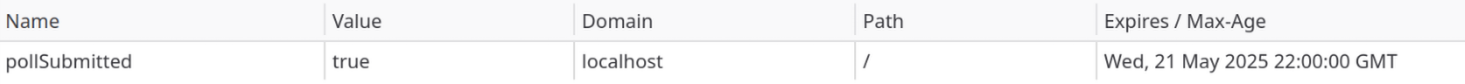
\includegraphics[width=0.9\textwidth]{pics/cookie.png} 
	\caption{Cookie stored in the browser} 
	\label{fig:cookie} 
\end{figure}\\ \\
The cookie is set only after the voting request is successfully processed. This order is crucial, as vote submissions can occasionally result in errors. If the cookie were set before confirmation, users could be wrongly prevented from resubmitting. By storing the cookie only after a successful vote, users can correct and resubmit their answers when needed.\\ \\
This method is not entirely secure. If someone knows where the cookie is stored and how to access it, they can delete it and vote again. Still, this setup addresses most common threats to the integrity of the poll.

\section{Results}
Results are arguably the most important feature of the application. Here, the voting data is displayed in a comprehensible way. This section of the platform includes the display of results depending on the different voting types — disclosed and anonymous — as well as an export option for further analysis of the voting data. 

\subsection{Backend}
The API for results consists of two main components. First, the total number of voters is calculated. This is done by counting the entries in the \textbf{UserPolls} table using Sequelize's \textbf{count} function. This number represents the total number of unique users who have participated in a specific poll. \\ \\
The second part handles the calculation of votes per question. For each question, the backend first determines the total number of answers submitted using the \textbf{UserAnswers} table. Then, for each answer within the question, it calculates the percentage of total votes that the answer received. These values are stored in an object named \textbf{questionVotes}, where each question id maps to another object containing answer ids and their corresponding vote percentages as strings formatted to two decimal places. \\
Weighted choice questions are also supported in the database and export. However, since each user can assign different weights to answers, it was not feasible to display this clearly in the frontend. Various methods were considered, such as showing the average or total weight per answer, but these either led to confusion or failed to reflect individual user input accurately. As a result, weight values are excluded from the visual results and are only available in the exported data.

\subsection{Frontend}
Figure \ref{fig:result} shows an example of a disclosed multiple choice question in the results view. For each question, the results section displays the list of possible answers along with the corresponding voting data. Depending on the poll's settings, the view can either show the percentage of total votes each answer received or a list of the users who voted for each answer.\\ \\
\begin{figure}[H] 
	\centering 
	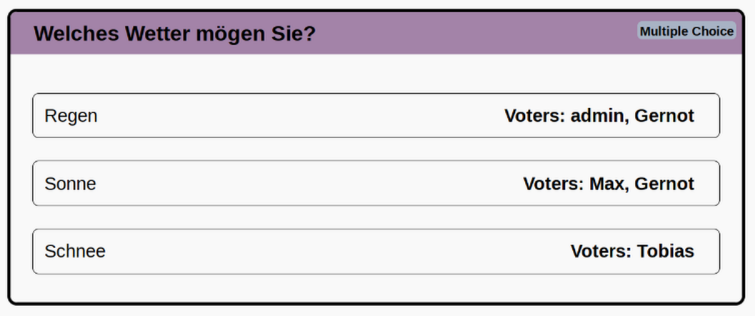
\includegraphics[width=0.9\textwidth]{pics/Results_example.png} 
	\caption{Example of result} 
	\label{fig:result} 
\end{figure}
The component uses two asynchronous API calls. The first fetches the overall voting results, using the API described in the backend part. The second fetches a list of voters per answer, if the poll is disclosed. This voter data is stored in an object where the keys are answer IDs and the values are arrays of usernames. \\ \\
A toggle button allows switching between the two display modes: percentages and voter names. This functionality is controlled by a boolean variable named \textbf{showVotersMode}. When \textbf{showVotersMode} is enabled, the result view shows the vote percentage for each answer. When disabled, it lists the names of the voters for each answer, or displays a fallback message if no one voted for that answer. \\ \\
The single-choice questions are displayed in the same format. Weighted choice questions are visually identical to multiple-choice ones, but their weight values are not shown due to the reasons mentioned earlier. Additional features include the optional display of the poll's image and description if such data is available. This ensures that the result view remains consistent with the poll's context.

\subsection{CSV-Export}
To allow for the further analysis and documentation of the poll results, a CSV export functionality was implemented. This export privides a structured overview of all user responses, including additional metrics such as the number of votes per answer and the average weight for weighted questions.\\ \\
The logic is handled in the \textbf{csvExportController.js} controller. Upon receiving a request, the system retrieves all relevant data for a given poll by its ID, including associated question, answers, and question types. The raw voting data is processed to count the number of responses per answer and to calculate the average weight if applicable. Special care is taken to distinguish between different types: for instance, "Single Choice" questions ensure that only one answer per user is counted, while "Weighted Choice" questions include the weight vale in the computation.\\ \\
The processed data is then converted into a structured CSV format using the json2csv library. The final file includes columns such as Poll Name, Question, Question Type, Answer, Vote Count and Average Weight, and can be downloaded directly by the user. This feature ensures transparency and enables further statistical evaluation using external tools like Excel.\parencite{json2csv}

\section{MyPolls}
\subsection{Purpose}
The "MyPolls" section is a central location in which users can view and manage all polls they have created. It provides access to the links for the polls as well as a delete option for them.
\subsection{Poll Link}
The link used for sharing the polls is generated by encoding key information into a hash. This is done using the "btoa" function, which creates a Base64-encoded string. In order to ensure compatibility with the browser URLs, the hash is also encoded using the "encodeURIComponent" function. The generated hash contains information about wether the poll is public, wether it is anonymous, the poll's mode and its ID.\parencite{mdn-btoa}\parencite{mdn-encodeUriComponent}\\\\
When a poll link is opened, the hash is first decoded using "decodeUriComponent" and then "atob". Depending on the mode specified in the url, the corresponding section in the dashboard is opened and the poll with the matching ID is loaded. Should the poll ID not exist in this specific mode, or in general, the system still opens the correct mode but in the default state without any poll selected.\parencite{mdn-atob}\parencite{mdn-decodeUriComponent}\\\\
To make sharing of the Surveys easier, a QR code generation was implemented. This was done using the React component "qrcode.react" which requires the link to the poll.\parencite{qrcode}
\subsection{Delete Polls}
The deletion of polls is crucial for two main reasons: first, to ensure that all associated data of a survey can be safely removed when necessary and second, to determine when a poll is still eligible for deletion. In this case, the deletion of polls is strictly limited to those that have not yet received any user votes. \\ \\
This constraint ensures the integrity of the data and avoids loss of user-generated information, which could distort statistical analysis or transparency within the system.\\ \\
To maintain data consistency, the deletion process is implemented as a transaction. This guarantees atomicity, meaning that either all steps of the deletion process succeed or none do - preventing partial data deletion and potential corruption. Sequelize's transaction management is used here to wrap the entire process in a rollback-safe structure. \parencite{sequelizedoku}

\paragraph{}
The deletion logic performs the following steps
\begin{enumerate}
	\item Validate that the poll exists.
	\item Fetch all related questions and their IDs.
	\item Check if any user answers exist for these questions. If so abort the operation with an error.
	\item Remove the many-to-many relations between answers from the "QuestionAnswers" table.
	\item Delete the associated answers.
	\item Delete the questions.
	\item Delete any group relations in the "PollGroups" table.
	\item Finally, delete the poll itself.
\end{enumerate}

\begin{figure}[h!]
\begin{code}
	const deletePoll = async (pollId) => {
		const transaction = await sequelize.transaction();
		try {
			...
			await PollGroups.destroy({
				where: { pollId },
				transaction,
			});
			await Polls.destroy({
				where: { id: pollId },
				transaction,
			});
			await transaction.commit();
			return { pollId, questionsDeleted: questionIds.length };
		} catch (error) {
			await transaction.rollback();
			throw error;
		}
\end{code}
\caption{Example for a Sequelize transaction}
\label{fig:delete_poll_code}
\end{figure}
Using Sequelize’s transaction mechanism not only helps to avoid data inconsistency, but also ensures that no information is accidentally deleted once users have participated in a poll. This feature is particularly important in environments where transparency and trust are key, such as in political or organizational voting systems.


\section{Accessibility}
\subsection{Tooltips}
To enhance the usability and user experience of the application, tooltips were integrated into all input field, providing users with contextual guidance and reducing the likelihood of input errors. For this purpose, the React library \textbf{react-tooltips} was utilized, offering a high degree of customizability in both design and behavior. This allowed for the implementation of consistent and informative tooltip elements throughout the interface.\parencite{tooltips}\\\\


Each from element is assigned a unique \textbf{data-tool-id}, which serves as a reference key within the central \textbf{Tooltips.js} configuration file. This file defines the content, styling, and interaction logic for each tooltip, ensuring that the visual presentation and timing behavior are consistent across the application. To prevent the tooltips from becoming distracting during regular use, a delay of 1500 milliseconds was introduced before displaying the tooltip on hover.\\\\


The overall purpose of this component was, to improve the intuitiveness of the application, especially for first-time users or those unfamiliar with specific input requirements.
\subsection{Screenreader}
\section{Styling}
\subsection{General styling}
At the beginning of the development process, a rough design was implemented to help visualize the overall concept of the future application. In order to maintain a clean and organized project structure, general styling files such as App.css, dashboard.css, voting.css, and others were placed within a dedicated styles directory.\\\\
The official styling of the application was done later in the making process, because only then it was demanded by the customers. The same applies to the color scheme which has two main colors: Yellow and Blackberry. In addition to the existing project structure, custom components such as the header with navigation and the footer were introduced, each of which can be individually styled. These were integrated to establish a layout that conforms to standard design practices.\\\\
To ensure consistency of the palette user defined characteristics from CSS where used to assign variables for each main color. \parencite{csscolorvariables}
\begin{figure}[h!]
	\begin{csscode}
		:root {
			--primary-color: #51184e;
			--secondary-color: #F9BB03;
			--primary-hover-color: rgb(163, 131, 168);
		}
	\end{csscode}
	\caption{Variables of the main colors}
	\label{fig:user_defined_characteristics}
\end{figure}

Those variables where then used in each element of where it was needed. Therefore changing the color scheme to a different one is less afford for the end user.

The basic structure of the page is split into three sections: header with navigation, main with content and footer with imprint and privacy policy. The style is based on the client's homepage therefore the standard background is purple but of the content it still is white to ensure readability. \parencite{lmppage}

\subsection{Responsive design}
Responsive design is essential nowadays because users access websites from a wide variety of devices - phones, tablets, laptops and desktops - each with different screen sizes and resolutions. It ensures a seamless, user-friendly experience across all platforms, which improve engagement and accessibility.\\ \\
To ensure responsiveness in each section of the application, "@media CSS at-rule" was used to apply different styles based on the screen size or device characteristics. This approach allows the layout, font sizes and element spacing to adapt dynamically, creating a smoother experience for users on any device. The navigation bar was designed with media queries to transform into so-called "burger menu" when the screen width falls below a certain threshold. This ensures usability on smaller devices like smartphones because the elements within the navigation get displayed in the menu now.
\begin{figure}[h!]
	\centering
	
\includegraphics[width=1\textwidth]{pics/navigation.png}
	\caption{Navigation}
	\label{fig:navigation}
\end{figure}
\begin{figure}[H]
	\centering
	
\includegraphics[width=0.3\textwidth]{pics/burger_menu.png}
	\caption{Burger menu}
	\label{fig:burger_menu}
\end{figure}
\subsection{Individual styling}
Some areas of the web application required additional styling efforts beyond the general layout to enhance usability, visual clarity and the overall aesthetic appearance. These areas were identified based on both internal testing and feedback from the client and were adapted to meet specific functional and visual needs.\\\\

Max Register

\paragraph{The Register Page} is a dedicated interface accessible exclusively to administrators. As seen in Figure \ref{fig:register_view}, the registration form is designed for clarity and ease of use. It features all necessary input fields to create a new user, alongside a dropdown for role selection. The description of the role is dynamically shown directly below depending on the selection, providing transparency about the permissions and purpose of each role. Styling is handled in the \textbf{register.css} file for modularity and maintainability.\\\\ 
\begin{figure}[H]
\centering
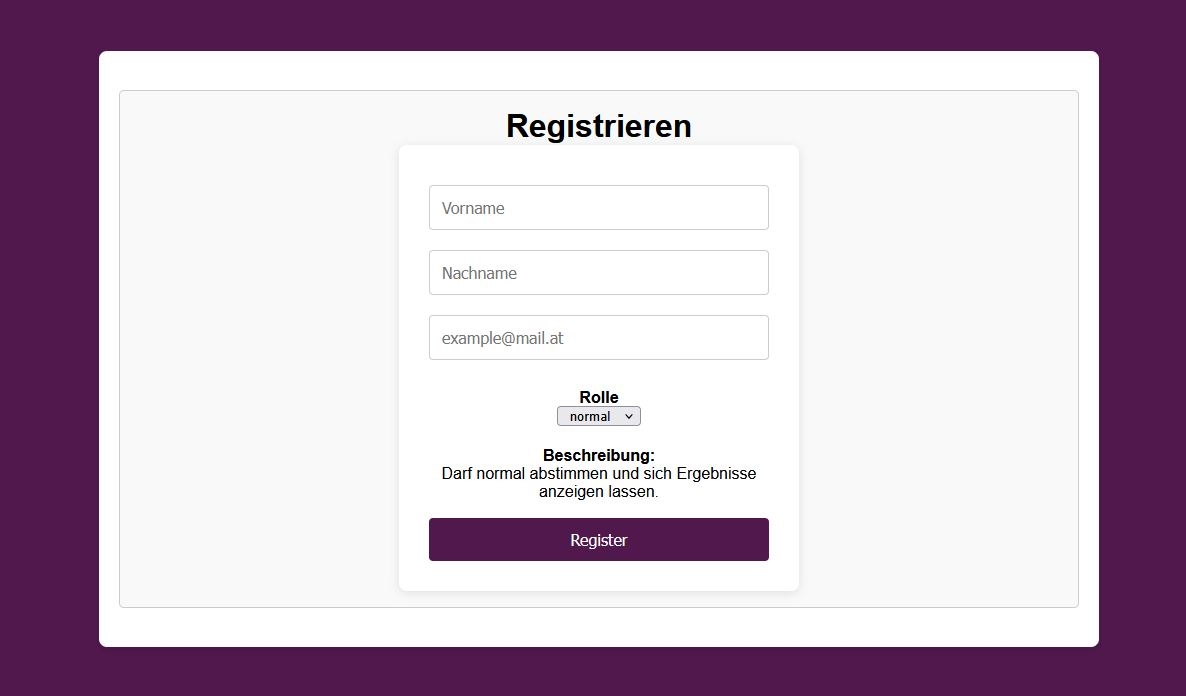
\includegraphics[width=0.9\textwidth]{pics/register_view.jpg}
\caption{Registration form}
\label{fig:register_view}
\end{figure}
\paragraph{Create Polls} allows users to configure and launch customized surveys. Due to the flexibility and number of inputs required, the styling and layout needed careful design considerations. The whole page has been divided into smaller parts, which are the metadata of the poll, survey type and group selection, image upload and the questions at the very end as a separate section. The Styling also had to be modular to support reusability in both the creation and editing interfaces.\\\\
\paragraph{Public and disclosed voting} Gernot Tobias
\paragraph{Results} Tobias
\paragraph{The Pollimage} enables users to create surveys with a title picture. It was styled to maintain visual harmony and responsiveness across Create, Voting, and Results views. The image container uses a flexbox layout to center the image horizontally, ensuring it looks balanced on all screen sizes. The image itself is limited to a maximum width of 90 percent of its container and a maximum height of 300 pixel to prevent oversized images from disrupting the layout. To preserve the original aspect ratio and avoid distortion, the \textbf{object-fit: contain} property is applied.\parencite{cssobjectfit}

\section{Deployment}
This project was deployed to test how it behaves in a live environment and to ensure that the setup can be easily replicated on other systems. Deployment also helps to verify that all components work together correctly outside of the development environment 
\subsection{Deployment Host}
For hosting the deployment, DigitalOcean was chosen. It allows you to create "droplets", which are virtual machines that can be configured with custom storage, RAM and other specifications. These droplets behave like personal servers but are hosted on the cloud and can be accessed publicly.
\subsubsection{Setup}
In our case, we used Ubuntu 22.04 LTS as the operating system. The server was configured with 25 GB of storage and 1 GB of RAM. After creating the "droplet", DigitalOcean assigned ab IP address to it, which makes it reachable over the internet. To configure and manage the server, we used SSH, allowing us to execute commands and install the necessary software remotely.
\subsection{Domain}
To enable HTTPS we decided to use a domain. We eventually aquired the domain “togema.eu” from the provider Namecheap.\\\\
On the Namecheap dashboard, a DNS record was added to point the domain name to the IP address of the "droplet" from DigitalOcean. After this configuration, the server is publicly accessible in any browser by using the domain name.
\subsection{Main Components}
Several core components were used to ensure that the server runs reliably, securely and efficiently. These components handle backend execution, traffic routing and HTTPS configuring.
\subsubsection{PM2 - Backend Process Manager}
To run the backend of the application on the server, we used \textbf{PM2}, a \textbf{Node.js} process manager. \textbf{PM2} ensures that the backend application continues running in the background even after the SSH session is closed, which is crucial for a web application, as you do not want to have to always maintain the session.\\\\
\textbf{PM2} also offers automatic restarts in case of crashes due to errors or unexpected shutdowns. It can log errors and process information, making it easier to monitor and maintain the server over time.
\subsubsection{Nginx- Web Server and Reverse Proxy}
To handle incoming traffic and route it properly, we used \textbf{Nginx} as a reverse proxy server. All requests to our domain are forwarded to the backend server running on \textbf{http://localhost:5000}.\\\\
Nginx also improves performance by efficiently managing multiple connections and reducing load on the backend. Additionally, it helps separate concerns by allowing us to manage routing, SSL, and load balancing in one place, while keeping the backend focused on application logic.
\begin{figure}[h!]
	\begin{terminal}
		server {
			listen 80;
			server_name domain_name www.domain_name;
			
			location / {
				proxy_pass http://localhost:5000;
				proxy_http_version 1.1;
				proxy_set_header Upgrade $http_upgrade;
				proxy_set_header Connection 'upgrade';
				proxy_set_header Host $host;
				proxy_cache_bypass $http_upgrade;
			}
		}
	\end{terminal}
	\caption{Example Nginx setup}
	\label{fig:user_defined_characteristics}
\end{figure}

\subsection{Certbot}
To enable HTTPS and secure data transmission, we used Certbot in combination with Nginx. Certbot is a tool provided by "Let's Encrypt" that automatically generates and installs SSL certificates on the server.\\\\
Once configured, Certbot not only sets up the SSL certificate but also updates the Nginx configuration to redirect HTTP traffic to HTTPS. This ensures that all communication between the client and the server is encrypted, improving both privacy and security for users accessing the application through the domain.

\chapter{Summary}

% Literaturverzeichnis
\printbibliography

% Abbildungsverzeichnis
\listoffigures
\newpage

\end{document}
